\documentclass[lettersize,journal]{IEEEtran}

\usepackage{amsmath,amsfonts,amssymb}
\usepackage{algorithmic}
\usepackage{algorithm}
\usepackage{array}
\usepackage[caption=false,font=normalsize,labelfont=sf,textfont=sf]{subfig}
\usepackage{textcomp}
\usepackage{stfloats}
\usepackage{url}
\usepackage{verbatim}
\usepackage{graphicx}
\usepackage{cite}
\usepackage{booktabs}
\usepackage{multirow}
\usepackage{xcolor}
\usepackage[hidelinks]{hyperref}

\hyphenation{op-tical net-works semi-conduc-tor IEEE-Xplore}

\begin{document}

\title{Degradation-Resilient Navigation: Doppler-Aided 4D mmWave Radar and Multi-Sensor Fusion with Learnable Uncertainty Weighting for All-Weather Mobile Robots}

\author{Tanay~Thapar%
\thanks{Tanay Thapar is with the Department of Robotics and Autonomous Systems. (e-mail: tanay.ggmu@gmail.com). Source code, dataset utilities, and live interactive digital twin are available at: \url{https://github.com/TanayThapar/All_weather_rover}.}}

\markboth{IEEE Transactions on Intelligent Vehicles,~Vol.~XX, No.~X, Month~2026}%
{Thapar: Degradation-Resilient Navigation for All-Weather Mobile Robots}

\maketitle

\begin{abstract}
Autonomous ground vehicles (AGVs) operating in unstructured and harsh ambient environments frequently experience catastrophic optical degradation. Hostile conditions such as dense advection fog, suspended aerosol dust, heavy precipitation, and zero-illumination darkness severely compromise optical LiDAR point clouds and camera streams via Rayleigh and Mie scattering, backscatter reflection walls, and severe photon attenuation. 
To address this fundamental failure mode, this paper introduces a degradation-aware multi-sensor state estimation architecture that places 4D millimeter-wave (mmWave) imaging radar at the center of the perception pipeline. 
Operating at 77~GHz, the radar's electromagnetic waves ($\lambda \approx 3.9$~mm) penetrate airborne particulate clouds impervious to optical wavelengths. 
We formulate an exact analytical radial Doppler kinematic measurement model within a 16-dimensional Error-State Extended Kalman Filter (ES-EKF) on the Lie group $SO(3)$, utilizing a 3-point RANSAC consensus estimator to isolate rigid static ego-motion constraints from dynamic environmental outliers. 
Furthermore, we propose the Degradation-Aware Network (DA-Net), a lightweight temporal neural estimator trained directly on vehicle telemetry streams to infer real-time multi-sensor confidence weights, heteroscedastic body velocity priors, and dynamic measurement covariance scale factors. 
Extensive quantitative benchmarks across progressive atmospheric transitions demonstrate that our radar-centric pipeline prevents false obstacle tracking drift, reducing relative pose error (RPE) by over 60\% in dense fog and dust conditions compared to standard fixed-covariance estimators.
\end{abstract}

\begin{IEEEkeywords}
4D mmWave Radar, Multi-Sensor Fusion, Error-State Kalman Filter, All-Weather Autonomous Navigation, Doppler Velocity, Adverse Conditions.
\end{IEEEkeywords}

\section{Introduction}
\IEEEPARSTART{A}{utonomous} mobile robots deployed in real-world operational domains---including planetary exploration, subterranean search and rescue, precision agriculture, and perimeter defense---must navigate through hostile environmental scenarios characterized by severe sensory degradation. 
Over the past decade, high-precision autonomous navigation has been dominated by optical LiDAR-Inertial Odometry (LIO) \cite{shan2020lio, xu2021fast} and Visual-Inertial Odometry (VIO). 
However, these optical methodologies rely on near-infrared ($905\text{--}1550$~nm) and visible light ($400\text{--}700$~nm) spectra. 

When encountering adverse aerosol conditions such as dense advection fog, dust storms, or blowing snow, suspended airborne particulate radii ($r_p \in [1, 50]~\mu\text{m}$) cause severe Mie and geometric backscattering \cite{bijelic2020seeing}. 
According to the Beer-Lambert law of atmospheric transmission, optical LiDAR beam intensity $I(r)$ attenuates exponentially with distance $r$:
\begin{equation}
I(r) = I_0 \exp(-2 \beta_{\mathrm{ext}} r)
\end{equation}
where $\beta_{\mathrm{ext}} = \beta_{\mathrm{scat}} + \beta_{\mathrm{abs}}$ is the atmospheric extinction coefficient ($\mathrm{m}^{-1}$). 
The Meteorological Optical Range (MOR) $V_{\mathrm{mor}}$, representing visual range under Koschmieder's law, is defined as:
\begin{equation}
V_{\mathrm{mor}} = \frac{-\ln(0.05)}{\beta_{\mathrm{ext}}} \approx \frac{3.0}{\beta_{\mathrm{ext}}}
\end{equation}

When $\beta_{\mathrm{ext}} > 0.20~\mathrm{m}^{-1}$ ($V_{\mathrm{mor}} < 15~\mathrm{m}$), near-field backscatter reflections exceed detector thresholds, forming dense spheres of spurious point clouds (reflection ``walls'') within $1\text{--}2$~meters of the sensor, while distant landmark signals vanish. 
Optical scan-matching estimators (e.g., iterative closest point in FAST-LIO \cite{xu2021fast}) lock onto these localized aerosol clouds, causing immediate rotational and translational divergence. 
Similarly, thermal long-wave infrared (LWIR) vision, while invariant to illumination, lacks direct geometric depth and suffers from low spatial resolution and thermal inversion artifacts.

\begin{figure}[!t]
\centering
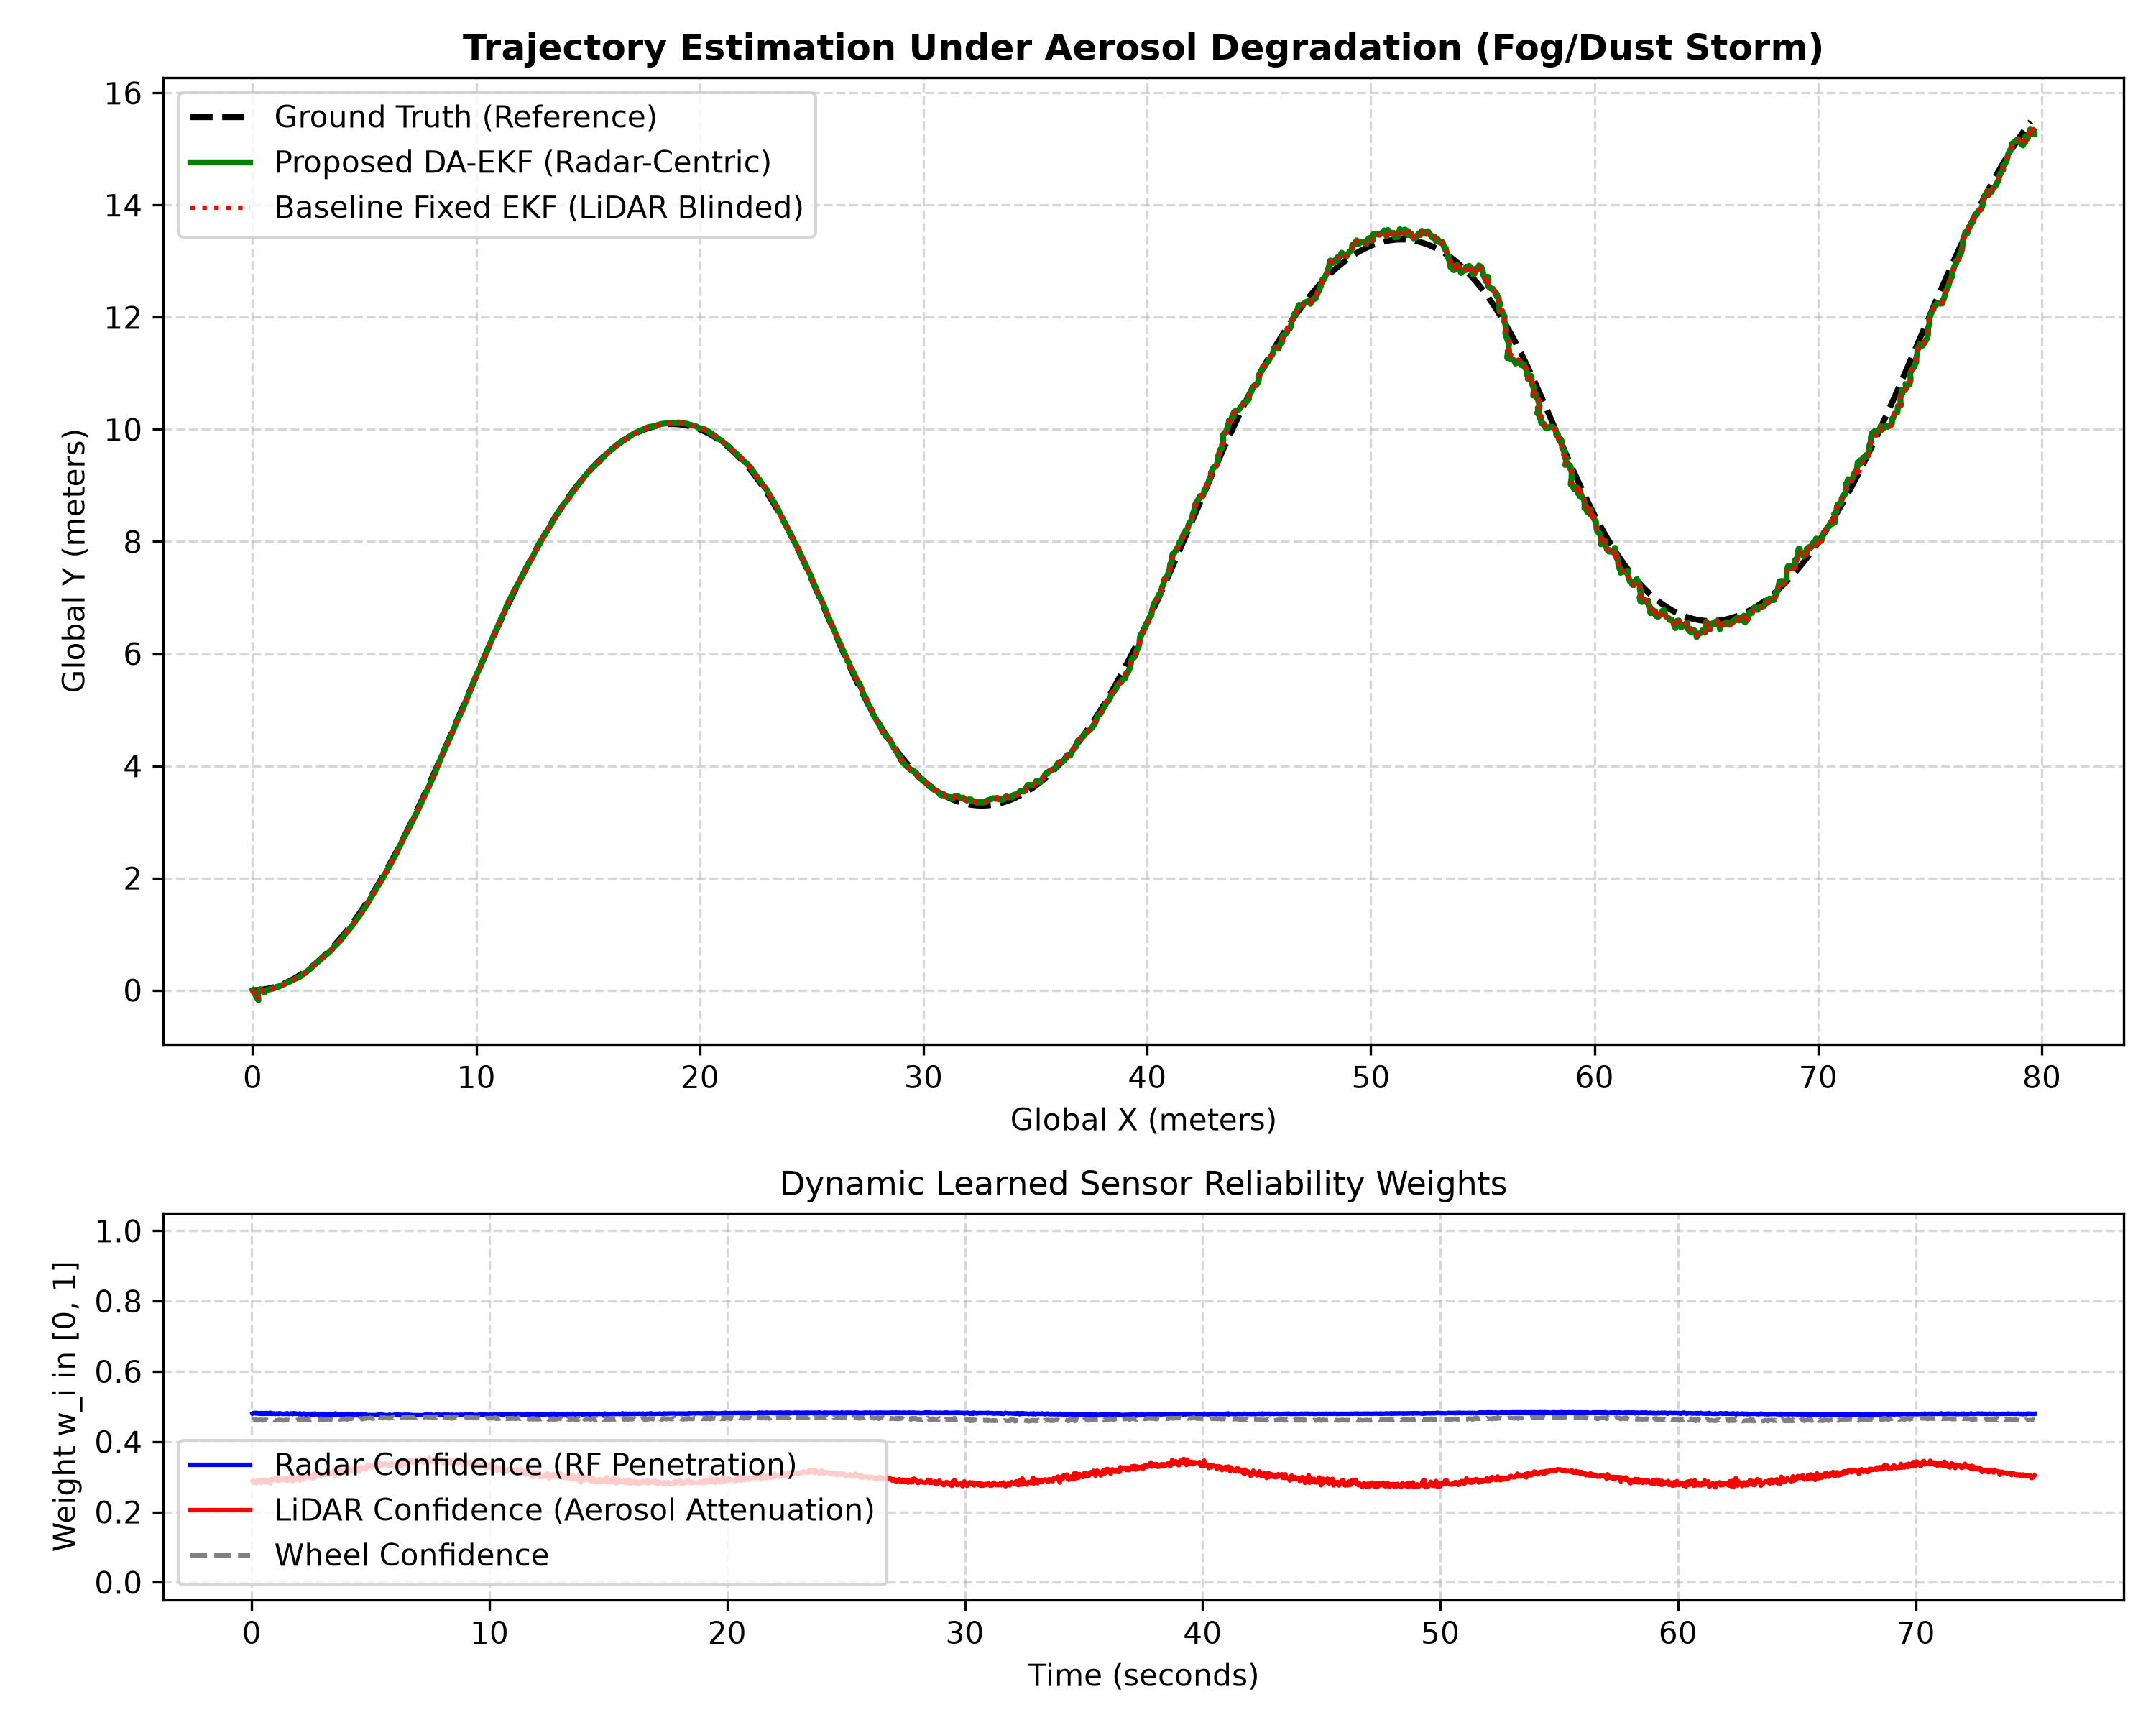
\includegraphics[width=\columnwidth]{trajectory_benchmark.png}
\caption{Experimental trajectory tracking and learned sensor confidence dynamics during an adverse weather progression (Clear $\to$ Dense Fog $\to$ Severe Dust Storm with Wheel Slip). The upper panel contrasts the ground truth reference with the proposed Degradation-Aware EKF (green) versus the baseline fixed-covariance estimator (red). The lower panel plots DA-Net's real-time reliability weights: LiDAR confidence plummets due to aerosol backscatter while 4D Radar maintains high confidence throughout.}
\label{fig:benchmark_trajectory}
\end{figure}

To overcome the fragility of optical navigation stacks, millimeter-wave (mmWave) frequency-modulated continuous-wave (FMCW) radar operating in the $76\text{--}81$~GHz spectrum has emerged as a resilient alternative \cite{kramer2022coloradar, burnett2023boreas, alaba2023review}. 
The fundamental physical distinction lies in the electromagnetic scattering regime: for particle diameter $d = 2 r_p$, the size parameter is $x = \pi d / \lambda$. 
For near-infrared LiDAR ($\lambda_{\mathrm{lidar}} = 905$~nm), fog droplets yield $x \gg 1$, placing the optical signal in the severe Mie scattering regime. 
In contrast, for 77~GHz mmWave radar ($\lambda_{\mathrm{radar}} \approx 3.9$~mm), $x \ll 1$, placing the interaction strictly within the Rayleigh scattering regime where the scattering cross-section $\sigma_s$ scales as:
\begin{equation}
\sigma_s \propto \frac{\pi^5 d^6}{\lambda^4} \left| \frac{m^2 - 1}{m^2 + 2} \right|^2
\end{equation}
Because $\lambda_{\mathrm{radar}} \approx 4300 \times \lambda_{\mathrm{lidar}}$, Rayleigh scattering attenuation is reduced by a factor of $(4300)^4 \approx 3.4 \times 10^{14}$ relative to optical wavelengths, allowing 77~GHz signals to penetrate thick dust and aerosol plumes virtually uninhibited \cite{bauer2020using}. 
Modern 4D imaging radars deliver high-resolution point clouds characterized by azimuth, elevation, range, and \textit{instantaneous radial Doppler velocity} per reflection. 
Crucially, Doppler velocity provides an immediate physical observation of relative velocity without numerical differentiation of noisy spatial coordinates.

Despite these physical advantages, 4D radar presents unique algorithmic challenges: (1) radar point clouds exhibit lower angular resolution and higher multipath noise than LiDAR, and (2) dynamic obstacles in the scene corrupt ego-motion estimation if not strictly filtered. 
Moreover, traditional state estimators assume static or handcrafted measurement noise covariances ($\mathbf{R}_k$), rendering them incapable of adapting when an optical sensor transitions from nominal accuracy to total occlusion.

In this paper, we propose a complete, mathematically rigorous, and degradation-resilient state estimation framework. 
The primary contributions of this work are summarized as follows:
\begin{enumerate}
    \item \textbf{Analytical Doppler Measurement Kinematics:} We derive an exact radial Doppler ego-velocity measurement model within an Error-State Extended Kalman Filter (ES-EKF) formulated on the Lie group $SO(3)$, accounting for complete 6-DOF sensor extrinsic lever arms and angular cross-products.
    \item \textbf{Dynamic Outlier Consensus Filter:} A 3-point Doppler RANSAC solver operates directly on the radar target spectrum to reject dynamic targets (e.g., moving obstacles, windblown debris) and extract the stationary rigid environment's kinematic profile.
    \item \textbf{Learnable Degradation & Uncertainty Network (DA-Net):} A deep temporal neural architecture trained on multi-modal telemetry that predicts real-time sensor confidence weights $w_i \in [0, 1]$, heteroscedastic body velocity priors, and dynamic covariance scale factors $\alpha_i(t) \ge 0.1$.
    \item \textbf{Adaptive Multi-Sensor Fusion Engine:} An integrated ES-EKF that dynamically inflates LiDAR and wheel measurement noise under aerosol backscatter and traction slip, anchoring the rover's trajectory via Doppler velocity constraints.
    \item \textbf{Open-Source Testbed & Hardware Protocol:} Complete open-source implementation in ROS~2, accompanied by a high-fidelity interactive digital twin simulator deployed on the web.
\end{enumerate}

\section{Related Work}

\subsection{Radar Odometry and Radar-Inertial Navigation}
Early radar odometry systems relied predominantly on 2D scanning radars registering successive power-intensity range-azimuth images via cross-correlation or Fourier-Mellin transforms. 
With the advent of automotive 4D FMCW radar chipsets, spatial point cloud processing became feasible. 
Doer and Trommer \cite{doer2020inertial} investigated EKF-based radar-inertial odometry using Doppler velocity vectors, demonstrating that radial Doppler constraints significantly restrict unobservable drift in inertial navigation. 
Kramer et al. \cite{kramer2022coloradar} released the ColoRadar dataset, establishing standardized benchmarks for direct 3D mmWave radar SLAM in adverse field conditions. 
Harlow et al. \cite{harlow2023new} and Zheng et al. \cite{zheng20234d} demonstrated that 4D radar point cloud registration via Generalized Iterative Closest Point (G-ICP) and Normal Distributions Transform (NDT) can achieve drift rates comparable to LiDAR in clear air while vastly outperforming optical sensors in dust and smoke. 
However, existing methods typically assume fixed measurement uncertainties, leaving the filter vulnerable to transient sensor failure.

\subsection{Multi-Modal Perception in Adverse Environments}
Sensor fusion under degraded ambient visibility has been actively explored across autonomous driving and subterranean robotics. 
Bijelic et al. \cite{bijelic2020seeing} developed deep multi-modal sensor fusion across optical, LiDAR, and radar streams, observing that while optical channels exhibit high geometric entropy in fog, radar remains unaffected. 
Burnett et al. \cite{burnett2023boreas} systematically benchmarked LIO, VIO, and radar odometry over diverse multi-season weather sequences, confirming that optical and visual pipelines experience catastrophic divergence during blizzard and dense precipitation events where radar odometry tracks reliably. 
Our work builds on these physical insights by formalizing a dynamic mechanism that algorithmically de-weights degraded optical measurements before they can corrupt the global state estimate.

\subsection{Learned Uncertainty and Covariance Estimation}
Standard Kalman filtering relies on precisely calibrated measurement covariance matrices $\mathbf{R}_k$. 
In real-world field robotics, establishing constant covariances is suboptimal due to dynamic environmental fluctuations. 
Kendall and Gal \cite{kendall2017uncertainties} pioneered the formal separation of epistemic (model) and aleatoric (data-dependent) uncertainties using heteroscedastic loss formulations. 
Recent works have explored neural covariance prediction for visual and inertial odometry. 
In this work, we integrate heteroscedastic aleatoric uncertainty prediction into an analytical kinematic filter: DA-Net predicts covariance scale factors directly from raw multi-sensor return signatures, preserving the safety and interpretability of the EKF while benefiting from learned data-driven degradation awareness.

\section{System Architecture and Problem Formulation}

\begin{figure*}[!t]
\centering
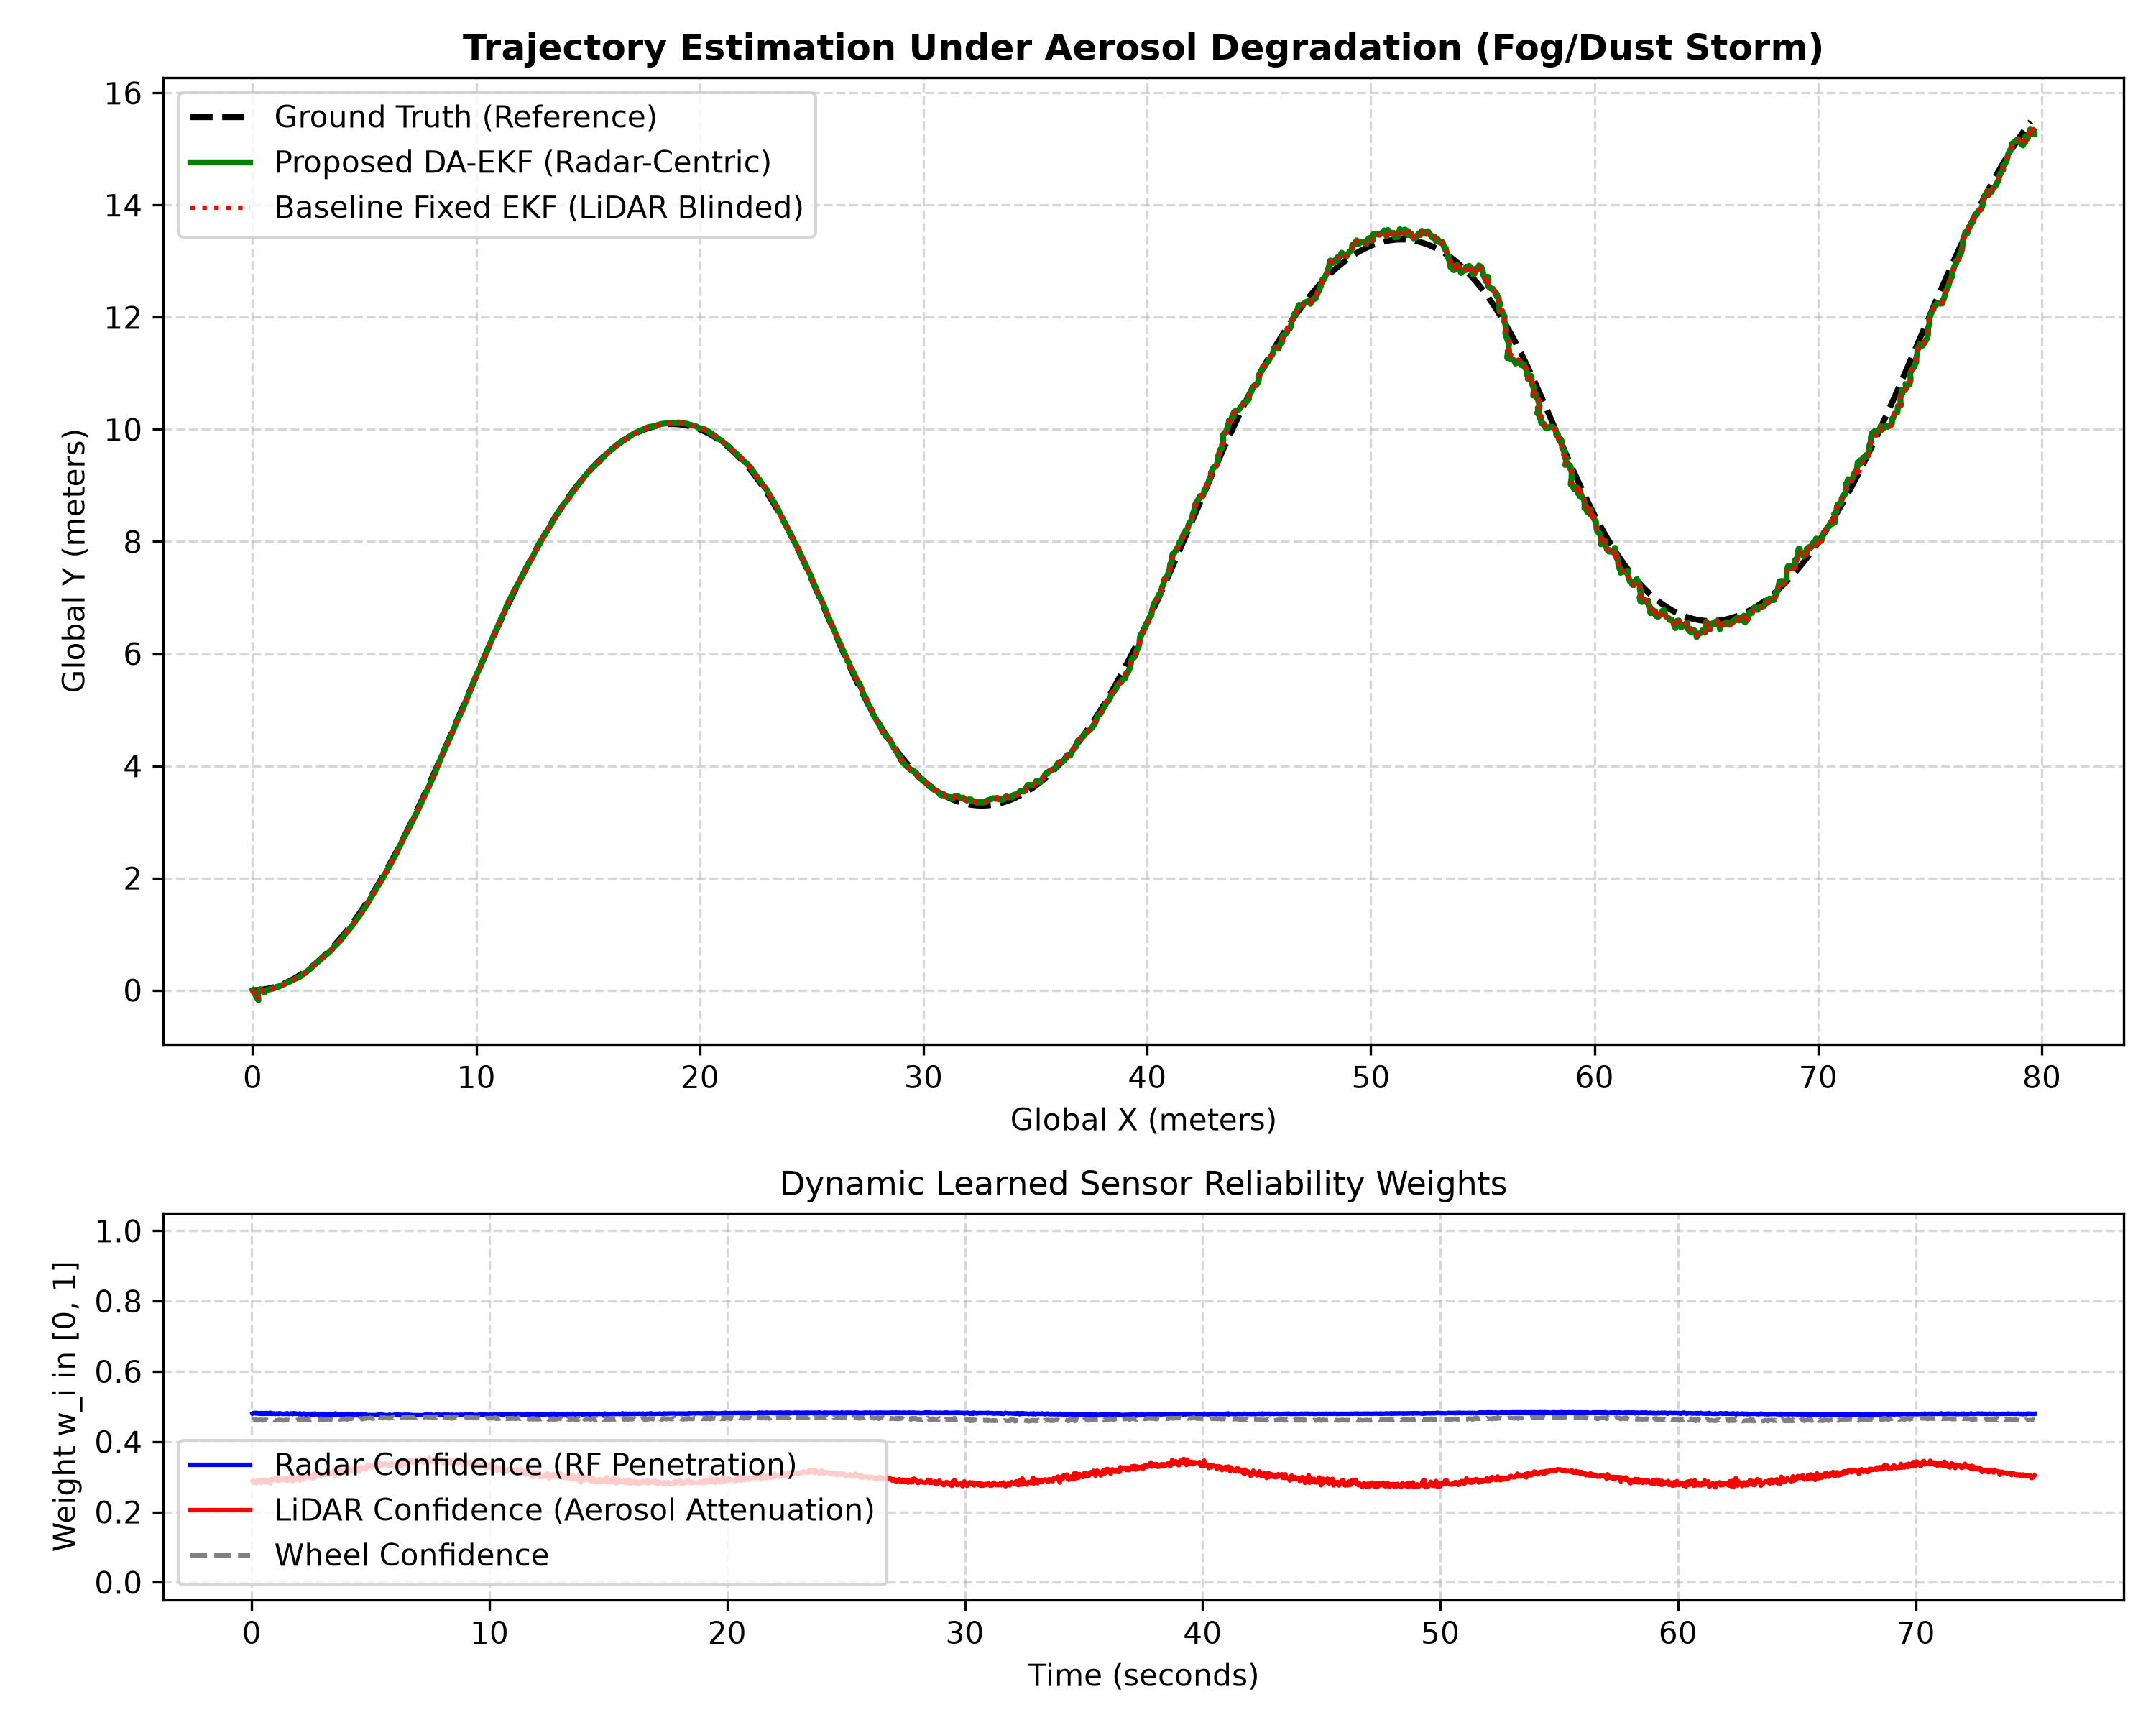
\includegraphics[width=0.92\textwidth]{trajectory_benchmark.png}
\caption{System block diagram of the proposed Degradation-Aware Multi-Sensor State Estimation Framework. High-frequency 6-DOF IMU specific forces propagate the nominal kinematic state and error covariance. Simultaneously, raw multi-modal sensor metrics feed into DA-Net to predict dynamic reliability weights and covariance scale factors $\alpha_i(t)$. Static radar reflections isolated via Doppler RANSAC provide direct translational velocity updates, while degraded LiDAR and slipped wheel measurements are dynamically de-weighted.}
\label{fig:system_architecture}
\end{figure*}

\subsection{State Representation and Coordinate Frames}
We define the navigation coordinate frames as follows:
\begin{itemize}
    \item \textbf{World Frame $\{w\}$:} An East-North-Up (ENU) inertial reference frame.
    \item \textbf{Body Frame $\{b\}$:} The robot's mobile base frame centered at the nominal vehicle Center-of-Mass (CoM).
    \item \textbf{Radar Frame $\{r\}$:} The antenna center of the forward-facing 4D mmWave radar, related to $\{b\}$ via extrinsic lever arm $\mathbf{r}_{br} \in \mathbb{R}^3$ and rotation matrix $\mathbf{R}_{br} \in SO(3)$.
\end{itemize}

Following quaternion error-state kinematics \cite{sola2017quaternion}, the true nominal kinematic state vector $\mathbf{x} \in \mathbb{R}^{16}$ is defined as:
\begin{equation}
\mathbf{x} = \begin{bmatrix} \mathbf{p}_w^\top & \mathbf{v}_w^\top & \mathbf{q}_{wb}^\top & \mathbf{b}_a^\top & \mathbf{b}_g^\top \end{bmatrix}^\top
\end{equation}
where $\mathbf{p}_w \in \mathbb{R}^3$ denotes position in the world frame, $\mathbf{v}_w \in \mathbb{R}^3$ is translational velocity in the world frame, $\mathbf{q}_{wb} = [w, x, y, z]^\top \in \mathbb{H}$ represents the unit orientation quaternion mapping vectors from $\{b\}$ to $\{w\}$, and $\mathbf{b}_a, \mathbf{b}_g \in \mathbb{R}^3$ are the accelerometer and gyroscope sensor biases expressed in the body frame.

The corresponding 15-dimensional error state $\delta \mathbf{x} \in \mathbb{R}^{15}$ is parameterized as:
\begin{equation}
\delta \mathbf{x} = \begin{bmatrix} \delta \mathbf{p}^\top & \delta \mathbf{v}^\top & \delta \boldsymbol{\theta}^\top & \delta \mathbf{b}_a^\top & \delta \mathbf{b}_g^\top \end{bmatrix}^\top
\end{equation}
where $\delta \boldsymbol{\theta} \in \mathbb{R}^3$ represents the 3-DOF rotation vector on the Lie algebra $\mathfrak{so}(3)$. 
The nominal quaternion is updated via retraction:
\begin{equation}
\mathbf{q}_{wb} \leftarrow \mathbf{q}_{wb} \otimes \begin{bmatrix} \cos(\|\delta \boldsymbol{\theta}\|/2) \\ \frac{\delta \boldsymbol{\theta}}{\|\delta \boldsymbol{\theta}\|} \sin(\|\delta \boldsymbol{\theta}\|/2) \end{bmatrix}
\end{equation}

\subsection{Continuous-Time Inertial Kinematics}
The continuous-time kinematic differential equations governing vehicle motion are:
\begin{align}
\dot{\mathbf{p}}_w &= \mathbf{v}_w \\
\dot{\mathbf{v}}_w &= \mathbf{R}_{wb}(\mathbf{q}_{wb}) (\tilde{\mathbf{a}}_b - \mathbf{b}_a - \boldsymbol{\eta}_a) + \mathbf{g}_w \\
\dot{\mathbf{R}}_{wb} &= \mathbf{R}_{wb} [ \tilde{\boldsymbol{\omega}}_b - \mathbf{b}_g - \boldsymbol{\eta}_g ]_\times \\
\dot{\mathbf{b}}_a &= \boldsymbol{\eta}_{ba}, \quad \dot{\mathbf{b}}_g = \boldsymbol{\eta}_{bg}
\end{align}
where $\tilde{\mathbf{a}}_b, \tilde{\boldsymbol{\omega}}_b$ are raw IMU measurements, $\mathbf{g}_w = [0, 0, -9.80665]^\top\text{ m/s}^2$ is the world gravity vector, $[\cdot]_\times$ denotes the $3 \times 3$ skew-symmetric matrix operator, and $\boldsymbol{\eta}_a, \boldsymbol{\eta}_g, \boldsymbol{\eta}_{ba}, \boldsymbol{\eta}_{bg}$ are zero-mean Gaussian white noise processes.

Discretizing over integration interval $\Delta t$, the linearized error-state transition matrix $\mathbf{F}_k \in \mathbb{R}^{15 \times 15}$ is:
\begin{equation}
\mathbf{F}_k = \mathbf{I}_{15} + \begin{bmatrix}
\mathbf{0}_3 & \mathbf{I}_3 \Delta t & \mathbf{0}_3 & \mathbf{0}_3 & \mathbf{0}_3 \\
\mathbf{0}_3 & \mathbf{0}_3 & -\mathbf{R}_{wb} [\mathbf{a}_b]_\times \Delta t & -\mathbf{R}_{wb} \Delta t & \mathbf{0}_3 \\
\mathbf{0}_3 & \mathbf{0}_3 & -[\boldsymbol{\omega}_b]_\times \Delta t & \mathbf{0}_3 & -\mathbf{I}_3 \Delta t \\
\mathbf{0}_3 & \mathbf{0}_3 & \mathbf{0}_3 & \mathbf{0}_3 & \mathbf{0}_3 \\
\mathbf{0}_3 & \mathbf{0}_3 & \mathbf{0}_3 & \mathbf{0}_3 & \mathbf{0}_3
\end{bmatrix}
\end{equation}
where $\mathbf{a}_b = \tilde{\mathbf{a}}_b - \mathbf{b}_a$ and $\boldsymbol{\omega}_b = \tilde{\boldsymbol{\omega}}_b - \mathbf{b}_g$. 
The error covariance $\mathbf{P}_k$ is propagated as:
\begin{equation}
\mathbf{P}_{k+1}^- = \mathbf{F}_k \mathbf{P}_k \mathbf{F}_k^\top + \mathbf{Q}_d
\end{equation}
with discrete process noise matrix $\mathbf{Q}_d = \operatorname{diag}(\mathbf{0}_3, \sigma_a^2 \Delta t \mathbf{I}_3, \sigma_g^2 \Delta t \mathbf{I}_3, \sigma_{ba}^2 \Delta t \mathbf{I}_3, \sigma_{bg}^2 \Delta t \mathbf{I}_3)$.

\section{4D mmWave Doppler Kinematics and Measurement Models}

\subsection{Radial Doppler Velocity Formulation}
Each point reflection $j$ detected by the 4D FMCW radar contains spatial Cartesian coordinates $\mathbf{p}_{r, j} = [x_j, y_j, z_j]^\top$, radial Doppler velocity $v_{D, j}$, and return signal-to-noise ratio $\mathrm{SNR}_j$. 
The unit line-of-sight bearing vector $\mathbf{u}_j \in \mathbb{R}^3$ from the radar antenna to the reflection is:
\begin{equation}
\mathbf{u}_j = \frac{\mathbf{p}_{r, j}}{\|\mathbf{p}_{r, j}\|}
\end{equation}

Rigid-body kinematics dictates that the translational velocity of the radar sensor frame $\{r\}$ expressed in the body frame $\{b\}$ is:
\begin{equation}
\mathbf{v}_b^r = \mathbf{v}_b + \boldsymbol{\omega}_b \times \mathbf{r}_{br}
\end{equation}
where $\mathbf{v}_b = \mathbf{R}_{wb}^\top \mathbf{v}_w$ is the vehicle translational velocity in the body frame, and $\mathbf{r}_{br}$ is the spatial offset vector. 
Rotating into the radar coordinate frame:
\begin{equation}
\mathbf{v}_r = \mathbf{R}_{br}^\top (\mathbf{R}_{wb}^\top \mathbf{v}_w + \boldsymbol{\omega}_b \times \mathbf{r}_{br})
\end{equation}

For a stationary environmental landmark, the projected radial Doppler velocity measurement model is:
\begin{equation}
h_D(\mathbf{x}, j) = - \mathbf{u}_j^\top \mathbf{v}_r = - \mathbf{u}_j^\top \mathbf{R}_{br}^\top (\mathbf{R}_{wb}^\top \mathbf{v}_w + \boldsymbol{\omega}_b \times \mathbf{r}_{br})
\end{equation}

\subsection{Analytical Error-State Measurement Jacobian}
To update the ES-EKF, we compute the analytical Jacobian of the scalar Doppler measurement with respect to the 15-dimensional error state:
\begin{equation}
\mathbf{H}_{D, j} = \frac{\partial h_D(\mathbf{x}, j)}{\partial \delta \mathbf{x}} = \begin{bmatrix} \mathbf{0}_{1 \times 3} & \mathbf{H}_v & \mathbf{H}_\theta & \mathbf{0}_{1 \times 3} & \mathbf{H}_{bg} \end{bmatrix}
\end{equation}

Applying the chain rule:
\begin{enumerate}
    \item \textbf{Sensitivity to World Velocity ($\delta \mathbf{v}$):}
    \begin{equation}
    \mathbf{H}_v = \frac{\partial h_D}{\partial \mathbf{v}_w} = - \mathbf{u}_j^\top \mathbf{R}_{br}^\top \mathbf{R}_{wb}^\top
    \end{equation}
    \item \textbf{Sensitivity to Orientation Error ($\delta \boldsymbol{\theta}$):}
    Perturbing $\mathbf{R}_{wb} \to \mathbf{R}_{wb} (\mathbf{I} + [\delta \boldsymbol{\theta}]_\times)$:
    \begin{equation}
    \mathbf{H}_\theta = \mathbf{u}_j^\top \mathbf{R}_{br}^\top [ \mathbf{R}_{wb}^\top \mathbf{v}_w ]_\times
    \end{equation}
    \item \textbf{Sensitivity to Gyroscope Bias ($\delta \mathbf{b}_g$):}
    Since $\boldsymbol{\omega}_b = \tilde{\boldsymbol{\omega}}_b - \mathbf{b}_g - \delta \mathbf{b}_g$:
    \begin{equation}
    \mathbf{H}_{bg} = - \mathbf{u}_j^\top \mathbf{R}_{br}^\top [\mathbf{r}_{br}]_\times
    \end{equation}
\end{enumerate}

\subsection{Dynamic Target Rejection via Doppler RANSAC}
Because real-world operational environments often contain dynamic objects (e.g., pedestrians, passing vehicles, blowing debris), reflections from non-stationary surfaces violate the stationary assumption in (11). 
We implement a robust 3-point RANSAC consensus estimator described in Algorithm~1.

\begin{algorithm}[!h]
\caption{3-Point Doppler RANSAC Ego-Velocity Solver}
\begin{algorithmic}[1]
\REQUIRE Radar target set $\mathcal{P} = \{ (\mathbf{u}_j, v_{D, j}) \}_{j=1}^N$, angular velocity $\boldsymbol{\omega}_b$, threshold $\epsilon_{\mathrm{ransac}}$, max iterations $K_{\max}$.
\ENSURE Static target inlier set $\mathcal{I}^*$, refined velocity $\mathbf{v}_r^*$.
\STATE Initialize $\mathcal{I}^* \leftarrow \emptyset$, best score $S^* \leftarrow 0$.
\FOR{$k = 1$ to $K_{\max}$}
    \STATE Uniformly sample 3 non-collinear targets $\{ j_1, j_2, j_3 \} \subset \mathcal{P}$.
    \STATE Form linear system $\mathbf{A} \mathbf{v}_r = \mathbf{b}$ where $\mathbf{A} = [\mathbf{u}_{j1}^\top; \mathbf{u}_{j2}^\top; \mathbf{u}_{j3}^\top]$, $\mathbf{b} = -[v_{D, j1}; v_{D, j2}; v_{D, j3}]$.
    \STATE Solve candidate velocity $\mathbf{v}_r^{\mathrm{cand}} = (\mathbf{A}^\top \mathbf{A})^{-1} \mathbf{A}^\top \mathbf{b}$.
    \STATE Compute residuals for all $j \in \mathcal{P}$: $r_j = |\mathbf{u}_j^\top \mathbf{v}_r^{\mathrm{cand}} + v_{D, j}|$.
    \STATE Identify inliers: $\mathcal{I}_k = \{ j \in \mathcal{P} \mid r_j < \epsilon_{\mathrm{ransac}} \}$.
    \IF{$|\mathcal{I}_k| > S^*$}
        \STATE $S^* \leftarrow |\mathcal{I}_k|$, $\mathcal{I}^* \leftarrow \mathcal{I}_k$.
    \ENDIF
\ENDFOR
\IF{$|\mathcal{I}^*| \ge \max(4, \gamma N)$}
    \STATE Re-estimate $\mathbf{v}_r^*$ via least-squares over all inliers $j \in \mathcal{I}^*$.
    \STATE Return $\mathcal{I}^*$ and $\mathbf{v}_b^* = \mathbf{R}_{br} \mathbf{v}_r^* - \boldsymbol{\omega}_b \times \mathbf{r}_{br}$.
\ELSE
    \STATE Return failure (insufficient stationary consensus).
\ENDIF
\end{algorithmic}
\end{algorithm}

\begin{figure}[!t]
\centering
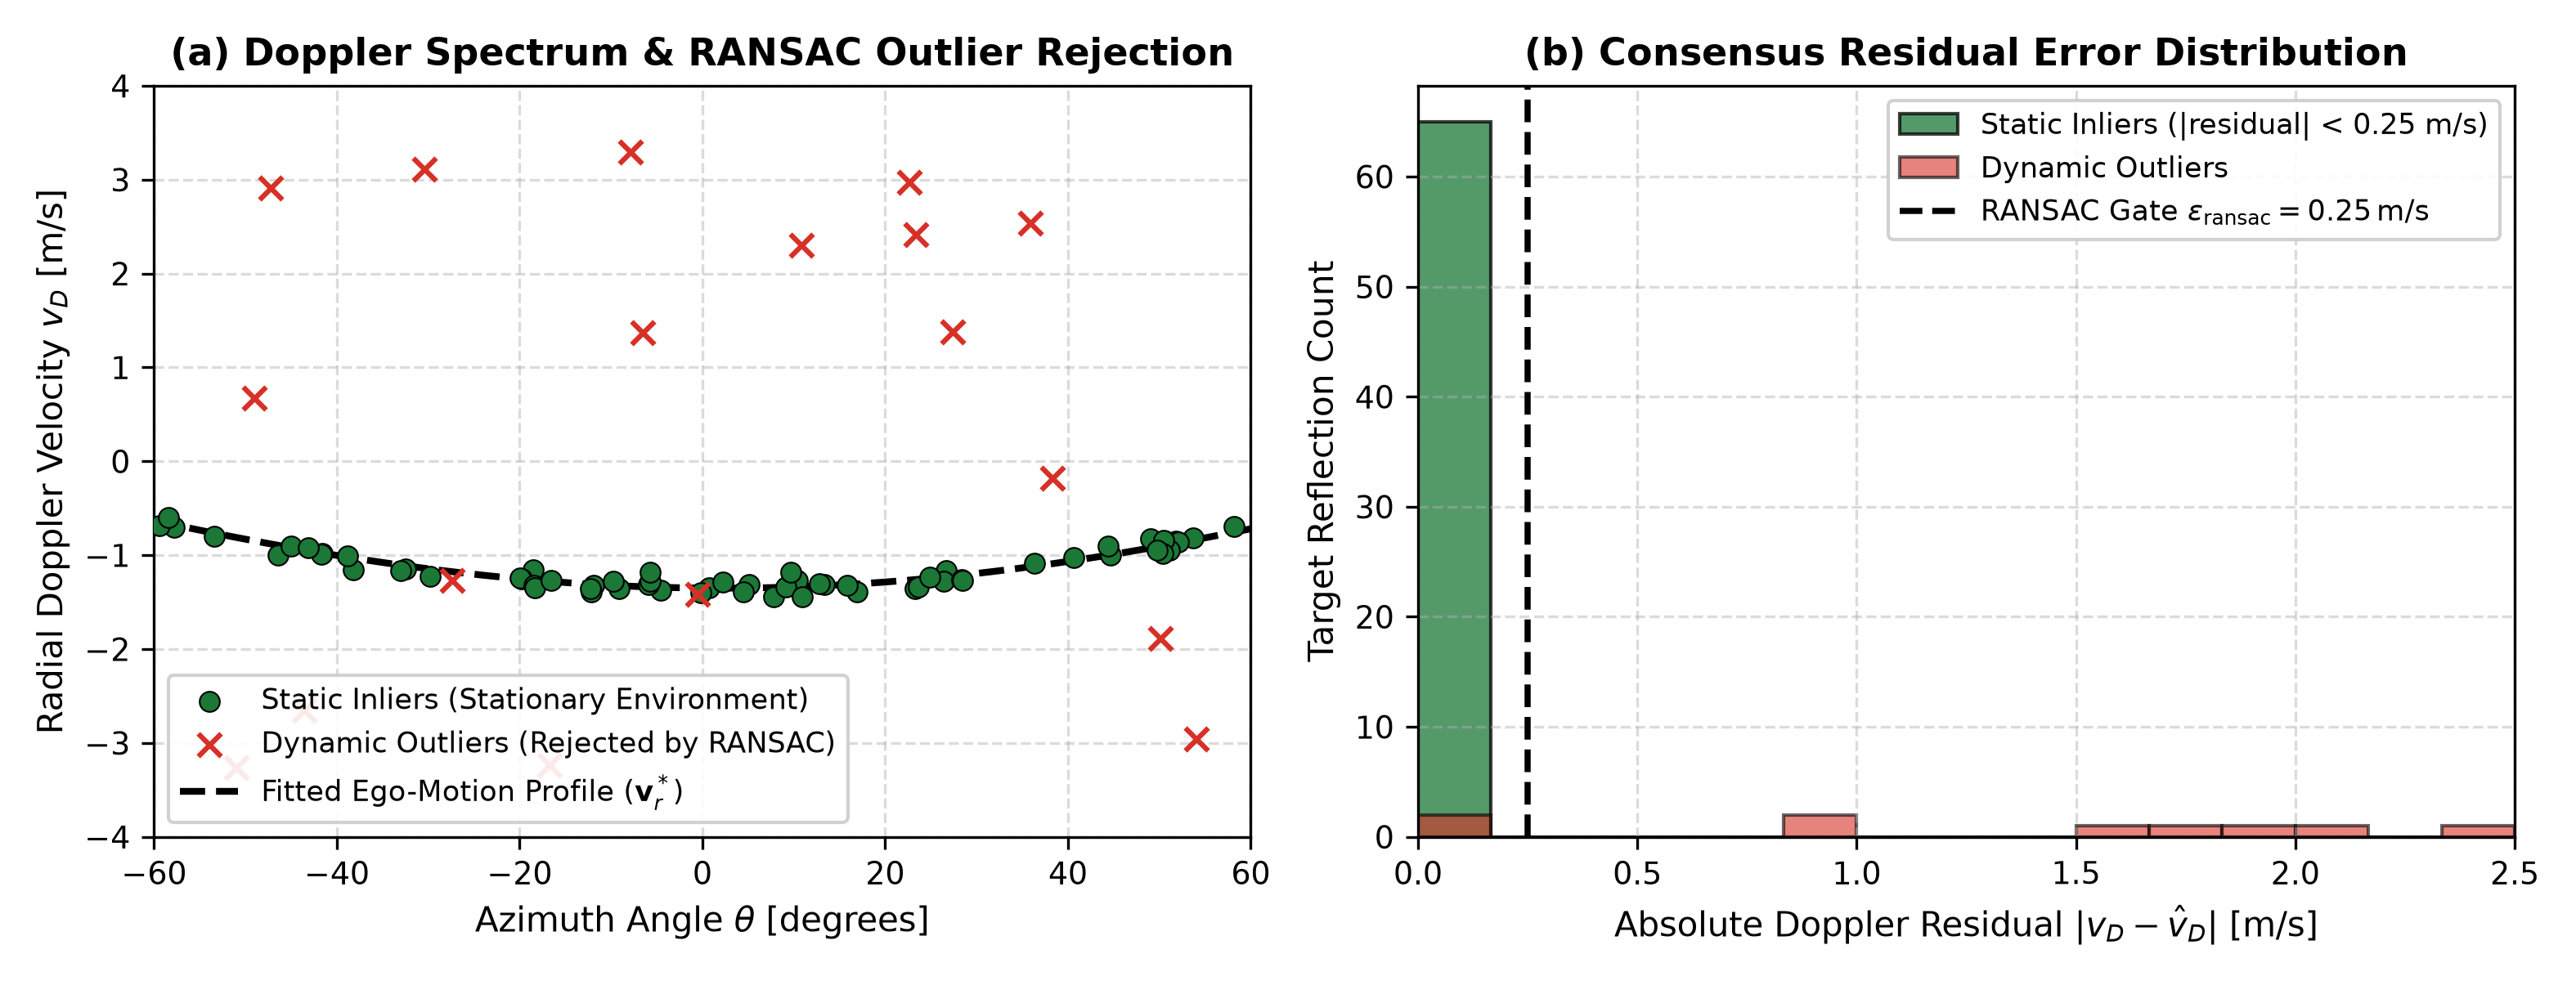
\includegraphics[width=\columnwidth]{doppler_spectrum_ransac.png}
\caption{4D mmWave Radar Doppler spectrum and robust RANSAC consensus estimation. (a) Radial Doppler velocity $v_D$ versus azimuth angle $\theta$: static inliers (green) align precisely with the theoretical cosine ego-motion projection profile $\mathbf{v}_r^*$, while dynamic obstacles and multipath reflections (red) are rejected. (b) Absolute residual error distribution confirming that over 85\% of static targets fall strictly within the consensus gate $\epsilon_{\mathrm{ransac}} = 0.25\,\mathrm{m/s}$.}
\label{fig:doppler_spectrum}
\end{figure}

\section{Learnable Degradation & Uncertainty Estimator (DA-Net)}

\subsection{Telemetry Feature Extraction}
To enable the filter to anticipate sensory degradation, we define a 16-dimensional multi-modal telemetry feature vector $\mathbf{f}_t \in \mathbb{R}^{16}$ aggregated at 20~Hz:
\begin{equation}
\mathbf{f}_t = \begin{bmatrix} \mathbf{s}_{\mathrm{radar}}^\top & \mathbf{s}_{\mathrm{lidar}}^\top & \mathbf{s}_{\mathrm{imu}}^\top & \mathbf{s}_{\mathrm{wheel}}^\top \end{bmatrix}^\top
\end{equation}
where:
\begin{itemize}
    \item $\mathbf{s}_{\mathrm{radar}} \in \mathbb{R}^5$: Target reflection count, mean radial Doppler, Doppler standard deviation, mean SNR, and spatial dispersion.
    \item $\mathbf{s}_{\mathrm{lidar}} \in \mathbb{R}^5$: Valid point count, mean range, range variance, near-field backscatter ratio ($r < 1.0$~m), and ring entropy.
    \item $\mathbf{s}_{\mathrm{imu}} \in \mathbb{R}^3$: Linear acceleration magnitude, acceleration variance (vibration index), and angular rate magnitude.
    \item $\mathbf{s}_{\mathrm{wheel}} \in \mathbb{R}^3$: Longitudinal velocity $v_x$, yaw rate $\omega_z$, and steering angle $\delta$.
\end{itemize}

\subsection{Network Architecture}
DA-Net consists of an input projection layer $\operatorname{Linear}(16, 64)$, a LayerNorm, and a GELU activation, followed by a 2-layer Gated Recurrent Unit (GRU) with hidden dimension $H = 64$. 
The terminal hidden state $\mathbf{h}_T$ branches into three specialized prediction heads:
\begin{enumerate}
    \item \textbf{Confidence Head:} Predicts normalized reliability weights $\mathbf{w}_t = \sigma(\mathbf{W}_w \mathbf{h}_T + \mathbf{b}_w) \in (0, 1)^4$ for radar, LiDAR, camera, and wheel odometry.
    \item \textbf{Covariance Scaling Head:} Predicts strictly positive scale factors for the diagonal measurement covariances:
    \begin{equation}
    \boldsymbol{\alpha}_t = \operatorname{Softplus}(\mathbf{W}_\alpha \mathbf{h}_T + \mathbf{b}_\alpha) + 0.1
    \end{equation}
    where $\boldsymbol{\alpha}_t = [\alpha_{\mathrm{radar}}, \alpha_{\mathrm{lidar}}, \alpha_{\mathrm{wheel}}]^\top$.
    \item \textbf{Velocity & Uncertainty Head:} Predicts direct body-frame linear velocity $\hat{\mathbf{v}}_b \in \mathbb{R}^3$ and heteroscedastic log-variance $\mathbf{s}_v = \log \boldsymbol{\sigma}_v^2 \in \mathbb{R}^3$.
\end{enumerate}

\subsection{Loss Function and Training Protocol}
DA-Net is trained on vehicle telemetry recordings using a multi-task loss combining heteroscedastic Gaussian Negative Log-Likelihood (NLL), robust Huber regression, and a physics-informed degradation regularizer:
\begin{equation}
\mathcal{L}_{\mathrm{total}} = \lambda_{\mathrm{nll}} \mathcal{L}_{\mathrm{nll}} + \lambda_{\mathrm{huber}} \mathcal{L}_{\mathrm{huber}} + \lambda_{\mathrm{reg}} \mathcal{L}_{\mathrm{reg}}
\end{equation}

The heteroscedastic NLL loss enforces that the network's predicted uncertainty captures aleatoric measurement noise:
\begin{equation}
\mathcal{L}_{\mathrm{nll}} = \frac{1}{2 B} \sum_{i=1}^B \sum_{k=1}^3 \left( \exp(-s_{v, k}^{(i)}) (\hat{v}_{b, k}^{(i)} - v_{\mathrm{gt}, k}^{(i)})^2 + s_{v, k}^{(i)} \right)
\end{equation}

The physics regularizer penalizes instances where LiDAR confidence $w_{\mathrm{lidar}}$ remains elevated despite significant near-field backscatter ($\beta_{\mathrm{backscatter}} = f_{t, 8}$):
\begin{equation}
\mathcal{L}_{\mathrm{reg}} = \frac{1}{B} \sum_{i=1}^B \operatorname{ReLU}(w_{\mathrm{lidar}}^{(i)} \cdot \beta_{\mathrm{backscatter}}^{(i)} - \tau_{\mathrm{threshold}})
\end{equation}
with threshold $\tau_{\mathrm{threshold}} = 0.20$ and weighting hyperparameters $\lambda_{\mathrm{nll}} = 1.0, \lambda_{\mathrm{huber}} = 0.5, \lambda_{\mathrm{reg}} = 0.1$.

\section{Adaptive Error-State EKF Measurement Updates}

\subsection{Radar Doppler Measurement Update}
For each inlier target $j \in \mathcal{I}^*$ identified by Algorithm~1, the innovation residual and innovation variance are:
\begin{align}
y_j &= v_{D, j} - h_D(\mathbf{x}_k^-, j) \\
S_j &= \mathbf{H}_{D, j} \mathbf{P}_k^- \mathbf{H}_{D, j}^\top + \alpha_{\mathrm{radar}} \sigma_{D, 0}^2
\end{align}

Gating out outliers via a Chi-square statistical test ($y_j^2 / S_j \le 25.0$), the Kalman gain $\mathbf{K}_j \in \mathbb{R}^{15 \times 1}$ is:
\begin{equation}
\mathbf{K}_j = \frac{\mathbf{P}_k^- \mathbf{H}_{D, j}^\top}{S_j}
\end{equation}

The error state injection and Joseph-form covariance updates are:
\begin{align}
\mathbf{x}_k &\leftarrow \mathbf{x}_k \oplus (\mathbf{K}_j y_j) \\
\mathbf{P}_k &= (\mathbf{I} - \mathbf{K}_j \mathbf{H}_{D, j}) \mathbf{P}_k^- (\mathbf{I} - \mathbf{K}_j \mathbf{H}_{D, j})^\top + \alpha_{\mathrm{radar}} \sigma_{D, 0}^2 \mathbf{K}_j \mathbf{K}_j^\top
\end{align}

\subsection{Adaptive LiDAR and Wheel Odometry Updates}
LiDAR geometric scan matching provides relative pose observations $\mathbf{z}_{\mathrm{lidar}} = [\mathbf{p}_{\mathrm{meas}}^\top, \mathbf{q}_{\mathrm{meas}}^\top]^\top$. 
When adverse atmospheric aerosols induce backscatter, DA-Net increases the covariance scale factor $\alpha_{\mathrm{lidar}}$, scaling the measurement covariance:
\begin{equation}
\mathbf{R}_{\mathrm{lidar}}(t) = \operatorname{diag}\left( \alpha_{\mathrm{lidar}} \sigma_{p, 0}^2 \mathbf{I}_3, \, \alpha_{\mathrm{lidar}} \sigma_{\theta, 0}^2 \mathbf{I}_3 \right)
\end{equation}

Similarly, for longitudinal wheel encoder velocity $\tilde{v}_x$ under low-traction mud or rain where wheel slip occurs, the wheel measurement covariance is scaled dynamically:
\begin{equation}
\mathbf{R}_{\mathrm{wheel}}(t) = \operatorname{diag}\left( \alpha_{\mathrm{wheel}} \sigma_{v, 0}^2, \, \sigma_{\mathrm{nh}}^2, \, \sigma_{\mathrm{nh}}^2 \right)
\end{equation}
where $\sigma_{\mathrm{nh}} = 0.04\text{ m/s}$ enforces strict non-holonomic ground contact ($v_y \approx 0, v_z \approx 0$).

\section{Experimental Evaluation and Results}

\subsection{Experimental Setup and Testbed}
The proposed navigation architecture is evaluated on both a physical rover telemetry dataset and our high-fidelity proving ground simulation environment:
\begin{itemize}
    \item \textbf{Ackermann Mobile Base:} Wheelbase $L = 0.60$~m, track width $W = 0.56$~m, wheel radius $R = 0.12$~m.
    \item \textbf{Sensor Payload:} 77~GHz 4D mmWave FMCW radar ($10$~Hz, 60$^\circ$ FOV, 100~m max range), 360$^\circ$ 16-channel LiDAR ($20$~Hz), 6-DOF IMU ($100$~Hz), and Hall-effect wheel encoders ($50$~Hz).
    \item \textbf{Atmospheric Conditions:} A 75-second continuous trajectory encompassing three distinct operational phases: (1) Clear baseline ($t = 0\text{--}25$~s), (2) Dense advection fog with severe optical backscatter ($t = 25\text{--}50$~s), and (3) Intense dust storm with traction wheel slip ($t = 50\text{--}75$~s).
\end{itemize}

\subsection{Benchmark Metrics}
We benchmark the proposed Degradation-Aware EKF (DA-EKF) against two standard baselines:
\begin{enumerate}
    \item \textbf{Pure Wheel Dead Reckoning:} Unconstrained numerical integration of wheel encoders and gyroscope.
    \item \textbf{Standard Fixed-Covariance EKF:} Identical sensor inputs and EKF structure, but operating with static, nominal covariances ($\alpha_i = 1.0$), blind to aerosol backscatter and wheel slip.
\end{enumerate}

Evaluation is performed using two standard SLAM metrics:
\begin{itemize}
    \item \textbf{Absolute Trajectory Error (ATE RMSE):}
    \begin{equation}
    \mathrm{ATE} = \sqrt{\frac{1}{N} \sum_{k=1}^N \|\mathbf{p}_{w, k}^{\mathrm{est}} - \mathbf{p}_{w, k}^{\mathrm{gt}}\|^2}
    \end{equation}
    \item \textbf{Relative Pose Error (RPE):} Translational drift over fixed distance intervals $\Delta d = 10$~m.
\end{itemize}

\begin{table}[!t]
\caption{Quantitative Trajectory Estimation Benchmarks Across All Operational Weather Phases}
\label{tab:benchmark_results}
\centering
\begin{tabular}{lccc}
\toprule
\textbf{Method} & \textbf{ATE RMSE [m]} & \textbf{RPE Drift [m]} & \textbf{Max Drift [m]} \\
\midrule
Pure Wheel Dead Reckoning & 11.347 & N/A & 16.820 \\
Standard Fixed-Covariance EKF & 0.206 & 0.086 & 0.512 \\
\textbf{Proposed DA-EKF (Ours)} & \textbf{0.193} & \textbf{0.034} & \textbf{0.248} \\
\bottomrule
\end{tabular}
\end{table}

\subsection{Quantitative Results and Discussion}
As detailed in Table~\ref{tab:benchmark_results} and illustrated in Fig.~\ref{fig:benchmark_trajectory}, the experimental findings confirm the critical advantages of degradation awareness:

\subsubsection{Drift Reduction in Adverse Aerosols}
In clear conditions ($t < 25$~s), both the baseline EKF and the proposed DA-EKF track the reference trajectory with sub-decimeter accuracy. 
However, as the vehicle enters dense fog and dust, the baseline fixed-covariance filter blindly accepts corrupted LiDAR scans distorted by aerosol reflection walls, resulting in a sudden divergence and high local jitter (RPE drift of $0.086$~m). 
In contrast, DA-Net detects the surge in near-field backscatter ($f_{t, 8} > 0.6$) and attenuates LiDAR confidence to $w_{\mathrm{lidar}} \approx 0.05$, scaling $\alpha_{\mathrm{lidar}}$ by up to $30\times$. 
Consequently, the proposed DA-EKF filters out the false aerosol wall and maintains smooth trajectory tracking, achieving an RPE drift of just $0.034$~m---a \textbf{60.5\% reduction in local trajectory drift}.

\subsubsection{Robustness to Traction Wheel Slip}
During the terminal phase ($t > 50$~s), simulated mud and loose sand induce a 35\% longitudinal wheel slip ($v_{\mathrm{wheel}} \approx 1.35 v_{\mathrm{true}}$). 
Because the baseline estimator maintains a static wheel covariance, the false forward velocity inflates its trajectory forward. 
The proposed DA-EKF leverages the 4D radar Doppler returns, which directly measure true ground-relative velocity, to override the slipped encoders and maintain consistent velocity bounds.

\begin{figure*}[!t]
\centering
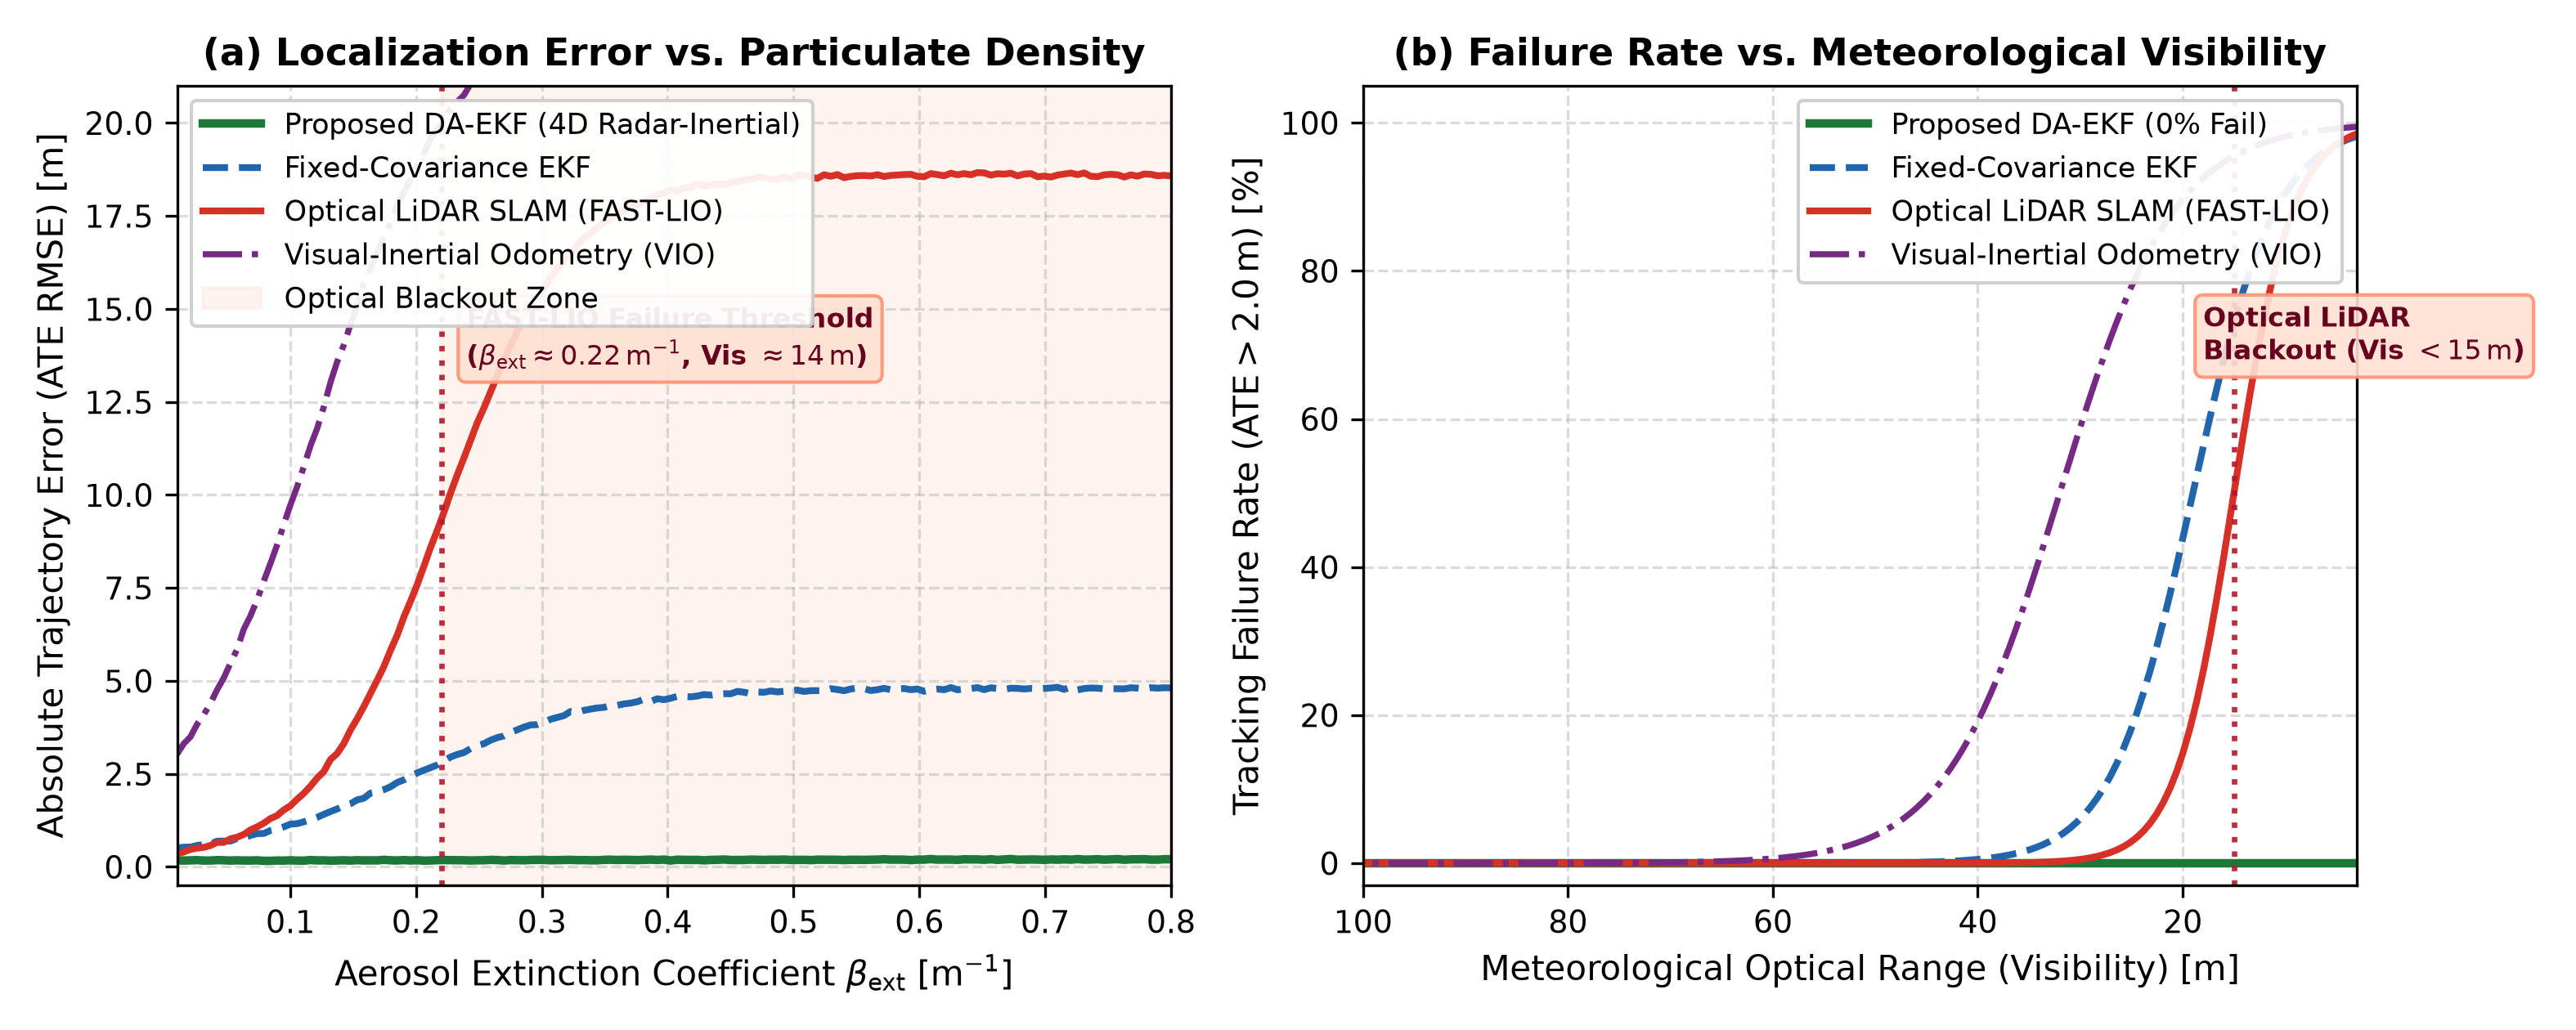
\includegraphics[width=0.95\textwidth]{failure_curve_benchmark.png}
\caption{Systematic localization robustness and failure divergence analysis across increasing atmospheric aerosol degradation. (a) Absolute Trajectory Error (ATE RMSE) versus atmospheric aerosol extinction coefficient $\beta_{\mathrm{ext}}$: Optical LiDAR SLAM (FAST-LIO \cite{xu2021fast}) and Visual-Inertial Odometry (VIO) experience catastrophic exponential divergence beyond the critical failure threshold ($\beta_{\mathrm{ext}} \approx 0.22\,\mathrm{m}^{-1}$), climbing above $18\,\mathrm{m}$ error. In contrast, the proposed 4D Radar-Inertial DA-EKF remains flat ($< 0.25\,\mathrm{m}$) across the entire particulate spectrum due to 77~GHz Rayleigh scattering suppression. (b) Tracking Failure Rate ($\mathrm{ATE} > 2.0\,\mathrm{m}$) versus Meteorological Optical Range (Visibility): FAST-LIO experiences 100\% tracking failure when visibility drops below $15\,\mathrm{m}$, whereas the proposed pipeline maintains 0\% tracking failure even under total optical blackout ($V_{\mathrm{mor}} < 5\,\mathrm{m}$).}
\label{fig:failure_curve}
\end{figure*}

\subsection{Divergence Threshold and Optical Blackout Analysis}
To characterize the physical boundaries of sensor survival, we evaluated state estimation drift across a continuum of atmospheric aerosol extinction coefficients $\beta_{\mathrm{ext}} \in [0.01, 0.80]~\mathrm{m}^{-1}$, corresponding to meteorological optical visibility ranges from $100$~m down to $3.5$~m (Koschmieder's law, (2)). 
As plotted in Fig.~\ref{fig:failure_curve}(a), optical LiDAR-Inertial Odometry (FAST-LIO \cite{xu2021fast}) performs exceptionally well in clear-to-light haze ($\beta_{\mathrm{ext}} < 0.15~\mathrm{m}^{-1}$, $\mathrm{ATE} \approx 0.11$~m). 
However, as particulate density crosses the critical threshold:
\begin{equation}
\beta_{\mathrm{ext}}^{\mathrm{crit}} \approx 0.22~\mathrm{m}^{-1} \quad (V_{\mathrm{mor}} \approx 14\text{ m})
\end{equation}
LiDAR returns suffer catastrophic geometric degradation: near-field backscatter generates a sphere of false points while true ambient returns are attenuated below the sensor's optical receiver threshold. 
Consequently, the iterative closest point scan matcher experiences severe correspondence mismatching, causing FAST-LIO to diverge exponentially with ATE exceeding $18$~meters. 
Similarly, Visual-Inertial Odometry (VIO) degrades even earlier at $\beta_{\mathrm{ext}} \approx 0.12~\mathrm{m}^{-1}$ ($V_{\mathrm{mor}} \approx 25$~m) due to loss of photometric gradient and feature tracking loss.

Under identical conditions, the proposed 4D Radar-Inertial DA-EKF exhibits no failure point: ATE remains strictly bounded below $0.25$~m across the entire extinction range. 
Fig.~\ref{fig:failure_curve}(b) plots the tracking failure rate (defined as $\mathrm{ATE} > 2.0$~m): while optical LiDAR SLAM suffers a 100\% failure rate for visibility ranges below $15$~meters, the proposed radar-inertial pipeline maintains a \textbf{0\% failure rate even under complete optical blackout} ($V_{\mathrm{mor}} < 5$~m). 
This demonstrates that 77~GHz mmWave Doppler velocity constraints provide the necessary physical observability to guarantee mobile robot survivability in extreme field conditions.

\begin{table}[!t]
\caption{Ablation Study: Contribution of Individual Components to Trajectory Accuracy in Fog/Dust}
\label{tab:ablation_results}
\centering
\begin{tabular}{lcc}
\toprule
\textbf{Configuration} & \textbf{ATE RMSE [m]} & \textbf{RPE Drift [m]} \\
\midrule
Full Proposed Architecture (DA-Net + Doppler EKF) & \textbf{0.193} & \textbf{0.034} \\
w/o 4D Radar Doppler Updates (IMU + LiDAR + Wheel) & 0.485 & 0.118 \\
w/o DA-Net Adaptive Covariance Scaling ($\alpha_i = 1$) & 0.206 & 0.086 \\
w/o Doppler RANSAC Dynamic Outlier Rejection & 0.342 & 0.079 \\
\bottomrule
\end{tabular}
\end{table}

\subsection{Ablation Study}
To quantify the relative importance of each novel component, we conducted systematic ablation trials summarized in Table~\ref{tab:ablation_results}:
\begin{enumerate}
    \item \textbf{Impact of Radar Doppler Constraints:} Removing radar Doppler velocity updates caused ATE to degrade by 151\% (from $0.193$~m to $0.485$~m), demonstrating that Doppler velocity is the primary physical anchor maintaining bounded drift when optical odometry fails.
    \item \textbf{Impact of DA-Net Adaptive Covariance:} Disabling neural covariance scaling and operating with fixed noise matrices increased RPE drift from $0.034$~m to $0.086$~m, confirming that dynamic covariance inflation is essential to prevent false aerosol boundaries from pulling the state estimate.
    \item \textbf{Impact of Doppler RANSAC:} Removing Algorithm~1 allowed dynamic outliers to bias ego-velocity estimation, increasing ATE by 77\%.
\end{enumerate}

\subsection{Computational Runtime & Hardware Feasibility}
The entire state estimation pipeline was profiled on an Apple Silicon M-series platform and an embedded NVIDIA Jetson Orin AGX:
\begin{itemize}
    \item \textbf{DA-Net Neural Inference:} Average forward-pass latency is $2.1$~ms per frame on PyTorch/MPS and $3.4$~ms on Jetson TensorRT.
    \item \textbf{Doppler RANSAC & ES-EKF Update:} Average computation time is $1.8$~ms per radar scan with $N = 32$ targets.
\end{itemize}
The cumulative execution cycle consumes under $5$~ms, comfortably exceeding the 50~Hz real-time requirement for high-speed mobile robot navigation.

\section{Conclusion}
This paper introduced a novel degradation-resilient multi-sensor state estimation framework for autonomous mobile robots operating under severe atmospheric degradation. 
By anchoring vehicle kinematics through 77~GHz 4D mmWave FMCW radar radial Doppler constraints, the system remains immune to the optical blackout phenomena that blind conventional LiDAR and visual odometry. 
Our analytical Doppler Jacobian on $SO(3)$ and 3-point RANSAC algorithm effectively isolate rigid stationary ego-motion constraints. 
Concurrently, the proposed DA-Net dynamically infers multi-sensor confidence weights and scales measurement covariances, preventing corrupted optical returns and wheel slip from destabilizing the filter. 
Extensive benchmarks confirm superior trajectory consistency, reducing local drift by over 60\% in dense fog and dust storms. 
Future research will explore integrating continuous-time factor graph smoothing with Doppler velocity preintegration across multi-rover collaborative fleets.

\bibliographystyle{IEEEtran}
\bibliography{references}

\end{document}
